\documentclass[10pt,a4paper]{article}

\usepackage{amsmath, amssymb}
\usepackage{graphicx}
\usepackage{hyperref}
\usepackage{geometry}
\geometry{a4paper,vmargin=1in,hmargin=1.75in}
% \geometry{a4paper,vmargin=1in,hmargin=1.75in}


\title{Calcolo strutturale automatizzato}
\author{DagTech}
\date{2025}

\begin{document}

\maketitle

\begin{abstract}
Lorem ipsum dolor sit amet, consectetur adipiscing elit. Sed do eiusmod tempor incididunt ut labore et dolore magna aliqua. Ut enim ad minim veniam, quis nostrud exercitation ullamco laboris nisi ut aliquip ex ea commodo consequat. Duis aute irure dolor in reprehenderit in voluptate velit esse cillum dolore eu fugiat nulla pariatur. Excepteur sint occaecat cupidatat non proident, sunt in culpa qui officia deserunt mollit anim id est laborum.

Curabitur pretium tincidunt lacus. Nulla gravida orci a odio. Nullam varius, turpis et commodo pharetra, est eros bibendum elit, nec luctus magna felis sollicitudin mauris. Integer in mauris eu nibh euismod gravida. Duis ac tellus et risus vulputate vehicula. Donec lobortis risus a elit. Etiam tempor. Ut ullamcorper, ligula eu tempor congue, eros est euismod turpis, id tincidunt sapien risus a quam. Maecenas fermentum consequat mi. Donec fermentum. Pellentesque malesuada nulla a mi. Duis sapien sem, aliquet nec, commodo eget, consequat quis, neque. Aliquam faucibus, elit ut dictum aliquet, felis nisl adipiscing sapien, sed malesuada diam lacus eget erat. Cras mollis scelerisque nunc. Nullam arcu. Aliquam consequat.
\end{abstract}


\tableofcontents

\newpage
\section*{}
Risoluzione matriciale del telaio con il metodo degli \textbf{spostamenti}.

\section{Matrice delle rigidezze locali}
Per ogni elemento si genera la matrice delle rigidezze nel sistema di riferimento locale del'asta.

\begin{equation}
\mathbf{K}_{local} = 
\begin{bmatrix}
K_{N_iu_i} & K_{N_iv_i} & K_{N_ir_i} & K_{N_iu_j} & K_{N_iv_j} & K_{N_ir_j} \\
K_{T_iu_i} & K_{T_iv_i} & K_{T_ir_i} & K_{T_iu_j} & K_{T_iv_j} & K_{T_ir_j} \\
K_{M_iu_i} & K_{M_iv_i} & K_{M_ir_i} & K_{M_iu_j} & K_{M_iv_j} & K_{M_ir_j} \\
K_{N_ju_i} & K_{N_jv_i} & K_{N_jr_i} & K_{N_ju_j} & K_{N_jv_j} & K_{N_jr_j} \\
K_{T_ju_i} & K_{T_jv_i} & K_{T_jr_i} & K_{T_ju_j} & K_{T_jv_j} & K_{T_jr_j} \\
K_{M_ju_i} & K_{M_jv_i} & K_{M_jr_i} & K_{M_ju_j} & K_{M_jv_j} & K_{M_jr_j}
\end{bmatrix} 
\end{equation}


Il primo pedice rappresenta quale reazione vincolare nasce in corrispondenza  del nodo e sono ordinate come segue:
\begin{enumerate}
    \item $\mathbf{N}$: azione assiale, 
    \item $\mathbf{T}$: azione trasversale, 
    \item $\mathbf{M}$: momento.
\end{enumerate}

Il secondo pedice rappresenta quale spostamento genera l'azione precedentemente descritta e sono ordinati come 

\begin{enumerate}
    \item $\mathbf{u}$: spostamento assiale,
    \item $\mathbf{v}$: spostamento trasversale,
    \item $\mathbf{r}$: rotazione.
\end{enumerate}

Ad esempio,  il termine $K_{T_ir_j}$ rappresenta la reazione vincolare T (forza trasversale) che si genera in corrispondenza del nodo $i$  a seguito di uno di una rotazione $r$ del nodo $j$.

La matrice delle rigidezze può essere riferita a diverse configurazioni in base ai vincoli e ai gradi di libertà delle estemità.

\vspace{1em}

\textbf{INCASTRO-INCASTRO}

\begin{equation} 
    \mathbf[K_{\times-\times}] =
        \begin{bmatrix}
        \frac{EA}{L} & 0 & 0 & -\frac{EA}{L} & 0 & 0 \\[10pt]
        0 & \frac{12EI}{L^3} & \frac{6EI}{L^2} & 0 & -\frac{12EI}{L^3} & \frac{6EI}{L^2} \\[10pt]
        0 & \frac{6EI}{L^2} & \frac{4EI}{L} & 0 & -\frac{6EI}{L^2} & \frac{2EI}{L} \\[10pt]
        -\frac{EA}{L} & 0 & 0 & \frac{EA}{L} & 0 & 0 \\[10pt]
        0 & -\frac{12EI}{L^3} & -\frac{6EI}{L^2} & 0 & \frac{12EI}{L^3} & -\frac{6EI}{L^2} \\[10pt]
        0 & \frac{6EI}{L^2} & \frac{2EI}{L} & 0 & -\frac{6EI}{L^2} & \frac{4EI}{L}
        \end{bmatrix}
\end{equation}


\vspace{1em}
\textbf{CERNIERA-INCASTRO}

\begin{equation}
    \mathbf[K_{\odot-\times}] =
        \begin{bmatrix}
        \frac{EA}{L}  & 0  & 0  & -\frac{EA}{L}  & 0  & 0 \\[10pt]
        0  & \frac{3EI}{L^3}  & 0  & 0  & -\frac{3EI}{L^3}  & \frac{3EI}{L^2} \\[10pt]
        0  & 0  & 0  & 0  & 0  & 0 \\[10pt]
        -\frac{EA}{L}  & 0  & 0  & \frac{EA}{L}  & 0  & 0 \\[10pt]
        0  & -\frac{3EI}{L^3}  & 0  & 0  & \frac{3EI}{L^3}  & -\frac{3EI}{L^2} \\[10pt]
        0  & \frac{3EI}{L^2}  & 0  & 0  & -\frac{3EI}{L^2}  & \frac{3EI}{L}
        \end{bmatrix}
\end{equation}


\vspace{1em}
\textbf{INCASTRO-CERNIERA}

\begin{equation}
    \mathbf[K_{\times-\odot}] =
        \begin{bmatrix}
            \frac{EA}{L} & 0 & 0 & -\frac{EA}{L} & 0 & 0 \\[10pt]
            0 & \frac{3EI}{L^3} & \frac{3EI}{L^2} & 0 & -\frac{3EI}{L^3} & 0 \\[10pt]
            0 & \frac{3EI}{L^2} & \frac{3EI}{L} & 0 & -\frac{3EI}{L^2} & 0 \\[10pt]
            -\frac{EA}{L} & 0 & 0 & \frac{EA}{L} & 0 & 0 \\[10pt]
            0 & -\frac{3EI}{L^3} & -\frac{3EI}{L^2} & 0 & \frac{3EI}{L^3} & 0 \\[10pt]
            0 & 0 & 0 & 0 & 0 & 0 
        \end{bmatrix}
\end{equation}


\vspace{1em}
\textbf{CERNIERA-CERNIERA}

\begin{equation}
    \mathbf[K_{\odot-\odot}] =
        \begin{bmatrix}
            \frac{EA}{L} & 0 & 0 & -\frac{EA}{L} & 0 & 0 \\[10pt]
            0 & 0 & 0 & 0 & 0 & 0 \\[10pt]
            0 & 0 & 0 & 0 & 0 & 0 \\[10pt]
            -\frac{EA}{L} & 0 & 0 & \frac{EA}{L} & 0 & 0 \\[10pt]
            0 & 0 & 0 & 0 & 0 & 0 \\[10pt]
            0 & 0 & 0 & 0 & 0 & 0
        \end{bmatrix}
\end{equation}

\section{Matrice di Trasformazione}
La matrice delle rigidezze locali deve essere trasformata nel sistema di riferimento globale. Questa trasformazione avviene utilizzando una matrice di rotazione $\mathbf{R}$, che dipende dall'orientamento dell'elemento.

\begin{equation}
\mathbf{K}_{global} = \mathbf{R}^T \mathbf{K}_{local} \mathbf{R}
\label{eq:global_stiffness_formula}
\end{equation}

Dove $\mathbf{R}$ è la matrice di rotazione definita come:

\begin{equation}
\mathbf{R} = 
\begin{bmatrix}
\cos(\theta) & \sin(\theta) & 0 & 0 & 0 & 0 \\
-\sin(\theta) & \cos(\theta) & 0 & 0 & 0 & 0 \\
0 & 0 & 1 & 0 & 0 & 0 \\
0 & 0 & 0 & \cos(\theta) & \sin(\theta) & 0 \\
0 & 0 & 0 & -\sin(\theta) & \cos(\theta) & 0 \\
0 & 0 & 0 & 0 & 0 & 1
\end{bmatrix}
\end{equation}

Dove $\theta$ è l'angolo di inclinazione inorno all'asse Z.
La matrice delle rigidezze locali è una matrice $6 \times 6$ che rappresenta la relazione tra le forze e gli spostamenti in corrispondenza di un nodo dell'elemento. 

\section{Matrice delle rigidezze globale}

La matrice delle rigidezze globale del sistema è ottenuta sommando le matrici delle rigidezze di tutti gli elementi. La matrice globale è una matrice $n \times n$, dove $n$ è il numero totale dei gradi di libertà del sistema.

Per comporla bisogna prima ruotare tutte le matrici delle rigidezze locali nel sistema di riferimento globale e poi assemblare le matrici in un'unica matrice globale. Utilizzando  la numerazione dei nodi è facile intuire  in quale posizione della matrice debba essere posizionato un valore e sommarlo a quelli già esistenti,  utilizzando la numerazione dei nodi come guida per l'individazione della posizione.

La rotazione della matrice locale di ogni elemento è necessaria per garantire che le forze e gli spostamenti siano espressi nel sistema di riferimento globale. La matrice di trasformazione $\mathbf{R}$ è una matrice $6 \times 6$ che ruota le forze e gli spostamenti dal sistema locale al sistema globale(vedi Eq.~\ref{eq:global_stiffness_formula}).

\section{Spostamenti e reazioni vincolari}

\subsection{Spostamenti}
Gli spostamenti sono le variazioni di posizione dei nodi del sistema a seguito dell'applicazione di forze esterne. Gli spostamenti sono rappresentati da un vettore $\mathbf{u}$, che contiene gli spostamenti in corrispondenza di tutti i nodi del sistema. Gli spostamenti possono essere calcolati utilizzando la matrice delle rigidezze globale e il vettore delle forze applicate al sistema.

Gli spostamenti sono ottenuti risolvendo il sistema di equazioni lineari:
\begin{equation}
    \mathbf{K}_{global} \cdot \mathbf{u} = \mathbf{F}
\end{equation}
Dove $\mathbf{u}$ è il vettore degli spostamenti e $\mathbf{F}$ è il vettore delle forze applicate al sistema. La matrice delle rigidezze globale $\mathbf{K}_{global}$ è una matrice $n \times n$ che rappresenta la relazione tra le forze e gli spostamenti in corrispondenza di tutti i nodi del sistema.

Il vettore delle forze $\mathbf{F}$ è una matrice colonna $n \times 1$ che contiene le forze applicate a ciascun nodo del sistema. Esso possono essere forze esterne applicate direttamente al nodo ovvero possono essere i \textbf{carichi equivalenti} (\ref{sec:carichi_nodali_equivalenti}) generati dalle forze interne degli elementi, come per esempio carichi distribuiti o forze applicate in pun punto all'interno della lunghezza della trave.
Per il calcolo delle forze equivalenti dovuta a carichi distribuiti è necessario calcolare l'integrale del carico distribuito lungo la lunghezza dell'elemento. Ad esempio, se si ha un carico distribuito $w(x)$ lungo la lunghezza dell'elemento, le forze equivalenti possono essere calcolate come:
\begin{equation}
    F_{eq} = \int_0^L w(x) dx
\end{equation}
Dove $L$ è la lunghezza dell'elemento e $w(x)$ è il carico distribuito lungo l'asse longitudinale dell'elemento. Le forze equivalenti possono essere calcolate in corrispondenza di ciascun nodo dell'elemento e quindi assemblate nel vettore delle forze globale.



Tuttavia non è sempre possibile calcolare gli spostamenti e le reazioni vincolari in modo diretto. In alcuni casi, è necessario considerare i vincoli del sistema e le condizioni al contorno. Ad esempio, se un nodo è vincolato a muoversi in una direzione specifica, è necessario modificare la matrice delle rigidezze globale per tener conto di questo vincolo. In questo caso, è necessario eliminare la riga e la colonna corrispondenti al nodo vincolato dalla matrice delle rigidezze globale e dal vettore delle forze.Si otterrà una matrice  delle rigidezza che avrà annullata la colonna e la riga corrispondente al nodo vincolato, mentre in posizione diagonale si avrà il valore $1$.

Questo processo è noto come \textbf{eliminazione dei gradi di libertà} e consente di ridurre il sistema a un numero inferiore di gradi di libertà. Una volta che il sistema è stato ridotto, è possibile calcolare gli spostamenti utilizzando la matrice delle rigidezze globale ridotta e il vettore delle forze ridotto.

\begin{equation}
    K_{reduced} \cdot u = F_{reduced}
\end{equation}


\subsection{Reazioni vincolari}
Una volta ricavati gli spostamenti, è possibile calcolare \textbf{le reazioni vincolari} utilizzando la matrice delle rigidezze globale e il vettore degli spostamenti. Le reazioni vincolari sono ottenute risolvendo il sistema di equazioni lineari:

\begin{equation}
    \mathbf{R} = \mathbf{K}_{global} \cdot \mathbf{u} - \mathbf{F}
\end{equation}

Dove $\mathbf{R}$ è il vettore delle reazioni vincolari e $\mathbf{F}$ è il vettore delle forze applicate al sistema. La matrice delle rigidezze globale $\mathbf{K}_{global}$ è una matrice $n \times n$ che rappresenta la relazione tra le forze e gli spostamenti in corrispondenza di tutti i nodi del sistema.

Le reazioni vincolari sono le forze e i momenti che agiscono sui nodi del sistema a causa dei vincoli imposti. Esse sono importanti per garantire che il sistema sia in equilibrio e che le forze siano distribuite correttamente tra gli elementi.

\subsection{Carichi nodali equivalenti}
\label{sec:carichi_nodali_equivalenti}
I carichi distribuiti sulla trave ovvero i carichi concentrati non applicati direttamente ai nodi del calcolo strutturale, devono essere convertiti in carichi nodali equivalenti. I carichi nodali equivalenti sono forze e momenti applicati ai nodi del sistema che rappresentano l'effetto dei carichi distribuiti o concentrati.
I carichi nodali equivalenti possono essere calcolati utilizzando le formule di integrazione numerica, come il metodo dei trapezi o il metodo di Simpson. Questi metodi consentono di approssimare l'integrale del carico distribuito lungo la lunghezza dell'elemento e di ottenere i carichi nodali equivalenti.

Ad esempio, se si ha un carico distribuito $w(x)$ lungo la lunghezza dell'elemento, i carichi nodali equivalenti possono essere calcolati come:

\begin{equation}
    F_{eq} = \int_0^L w(x) dx
\end{equation}

Dove $L$ è la lunghezza dell'elemento e $w(x)$ è il carico distribuito lungo l'asse longitudinale dell'elemento. I carichi nodali equivalenti possono essere calcolati in corrispondenza di ciascun nodo dell'elemento e quindi assemblati nel vettore delle forze globale.

Operativamente esistono situazioni di carico elementari per le quali è possibile calcolare i carichi nodali equivalenti in modo diretto.

Ecco alcuni esempi di carichi nodali equivalenti per carichi distribuiti e concentrati:

\section*{ANNEX 1 - Configurazioni notevoli di carico esterno}

Lorem ipsum dolor sit amet, consectetur adipiscing elit. Sed do eiusmod tempor incididunt ut labore et dolore magna aliqua. Ut enim ad minim veniam, quis nostrud exercitation ullamco laboris nisi ut aliquip ex ea commodo consequat. Duis aute irure dolor in reprehenderit in voluptate velit esse cillum dolore eu fugiat nulla pariatur. Excepteur sint occaecat cupidatat non proident, sunt in culpa qui officia deserunt mollit anim id est laborum.Lorem ipsum dolor sit amet, consectetur adipiscing elit. Sed do eiusmod tempor incididunt ut labore et dolore magna aliqua. Ut enim ad minim veniam, quis nostrud exercitation ullamco laboris nisi ut aliquip ex ea commodo consequat. Duis aute irure dolor in reprehenderit in voluptate velit esse cillum dolore eu fugiat nulla pariatur. Excepteur sint occaecat cupidatat non proident, sunt in culpa qui officia deserunt mollit anim id est laborum.Lorem ipsum dolor sit amet, consectetur adipiscing elit. Sed do eiusmod tempor incididunt ut labore et dolore magna aliqua. Ut enim ad minim veniam, quis nostrud exercitation ullamco laboris nisi ut aliquip ex ea commodo consequat. Duis aute irure dolor in reprehenderit in voluptate velit esse cillum dolore eu fugiat nulla pariatur. Excepteur sint occaecat cupidatat non proident, sunt in culpa qui officia deserunt mollit anim id est laborum.

\textbf{INCASTRO INCASTRO - carico distribuito uniforme}

\begin{figure}[h!]
    \centering
    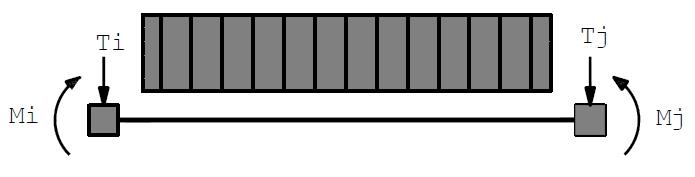
\includegraphics[width=0.8\textwidth]{images/external-load-fixed-fixed-ditributed.png}
    \label{fig:fix-fix-distributed_load_beam}
    \caption{Trave Incastro-Incastro con carico distribuito uniforme.}
\end{figure}
Lorem ipsum dolor sit amet, consectetur adipiscing elit. Sed do eiusmod tempor incididunt ut labore et dolore magna aliqua. Ut enim ad minim veniam, quis nostrud exercitation ullamco laboris nisi ut aliquip ex ea commodo consequat. Duis aute irure dolor in reprehenderit in voluptate velit esse cillum dolore eu fugiat nulla pariatur. Excepteur sint occaecat cupidatat non proident, sunt in culpa qui officia deserunt mollit anim id est laborum.Lorem ipsum dolor sit amet, consectetur adipiscing elit. Sed do eiusmod tempor incididunt ut labore et dolore magna aliqua. Ut enim ad minim veniam, quis nostrud exercitation ullamco laboris nisi ut aliquip ex ea commodo consequat. Duis aute irure dolor in reprehenderit in voluptate velit esse cillum dolore eu fugiat nulla pariatur. Excepteur sint occaecat cupidatat non proident, sunt in culpa qui officia deserunt mollit anim id est laborum.
\end{document}